%\documentclass[a6paper]{article}   % smartphone
\documentclass[17pt]{extarticle}  % print quality
\usepackage{polyglossia}
\usepackage[margin=20mm]{geometry}
\setdefaultlanguage{marathi}
\setotherlanguages{english}
%\textbf with "Sanskrit Text" produces the shape warning because the default Sanskrit Text font on Windows does not have a bold equivalent; try Yashomudra or Shobhika; now I like Tiro better
\newfontfamily\devanagarifont[Script=Devanagari]{Sanskrit Text}
%\newfontfamily\devanagarifont[Script=Devanagari]{Tiro Devanagari Marathi}
\newfontfamily\englishfont{Georgia}

%\pagenumbering{gobble}
\setlength{\parindent}{0pt}% Remove paragraph indent
\usepackage[skip=\medskipamount]{parskip}
\usepackage{fontawesome}
\usepackage[style=english]{csquotes}
\usepackage{verse}
\usepackage{xcolor}
\usepackage{graphics}
\usepackage{hyperref}
\hypersetup{
    colorlinks=true,
    linkcolor=blue,
    filecolor=magenta,
    citecolor=blue,
    urlcolor=purple,
}

% control hyphenation: https://tex.stackexchange.com/a/177179/64425
\tolerance=1
\emergencystretch=\maxdimen
\hyphenpenalty=10000
\hbadness=10000
% control hyphenation: https://tex.stackexchange.com/a/177179/64425

\begin{document}

\title{साखरेची पुरणपोळी}
\author{केदार म्हसवडे}
\date{पुणे, २ नोव्हेंबर् २०२३}
\maketitle
\hrule
\vspace{5mm}
ही कृती मी माझी पत्नी दीपा जोशी आणि सासूबाई कुंदा जोशी (अहो-आई) यांच्याकडून शिकलो आहे. इतक्या वेळा मी ही मूर्तिमंत महाराष्ट्रियन् नजाकत प्रत्यक्ष घडताना पाहिली आहे की मला ती शिकणे भाग होते. माझं वैयक्तिक (आणि म्हणूनच काहीसं विक्षिप्त) मत असं आहे की ही पुरणपोळी सर्व गोड मराठी पदार्थांची गॉड आहे! अहो-आईंनी ही पुरणपोळी आजवर निदान ९०-१०० वेळा केली असेल असा माझा अंदाज आहे. 

काही चोखंदळ लोक पुरणपोळीचं पुरण म्हणजे गुळाचं असं म्हणतात आणि पुरण साखरेचं केलं की नाकं मुरडतात. त्यांनी आजपर्यंत खाल्लेल्या रुचीचा तो परिणाम असेल, पण असं वज्रलेप मत असायलाच पाहिजे असं नाही. नागपूरकडे होणारी ही पुरणपोळी इतकी सुंदर होते की अगदी कट्टर गुळाचं पुरण आवडणाऱ्यांच्या तोंडाला देखील पाणी सुटल्याशिवाय राहणार नाही! जर तसं झालंच तर ते मान्य करण्याचा प्रामाणिकपणा हवा मात्र.

मी ही कृती पूर्णपणे टाइप्-सेट् करायचं ठरवलं आहे, पण एकदा ती हस्ताक्षरात लिहून काढली, म्हणजे बरेच दिवस ती लिहीत होतो (इतकं की दीपा म्हणायची, \enquote{झालं का तुझं पुरणपोळीच्या कृतीचं \enquote{पुस्तक} लिहून?}). तूर्तास पूर्ण कृती हस्ताक्षरातच वाचा, काही दिवसांनी टाइप्-सेट् करीन. 

नक्की करा ही पुरणपोळी आणि समाधानाचे मळे फुलवा! आणि थोडंसं \enquote{आयतं} खावंसं वाटत असेल तर मला सांगा, मी तुमच्यासाठी करीन!

\begin{figure}[h!]
    \centering
    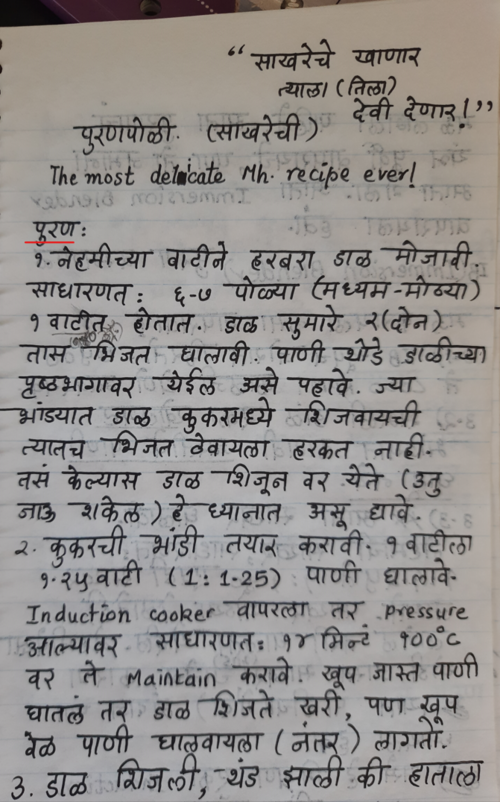
\includegraphics{img/01-s.png}
\end{figure}
\begin{figure}[h!]
    \centering
    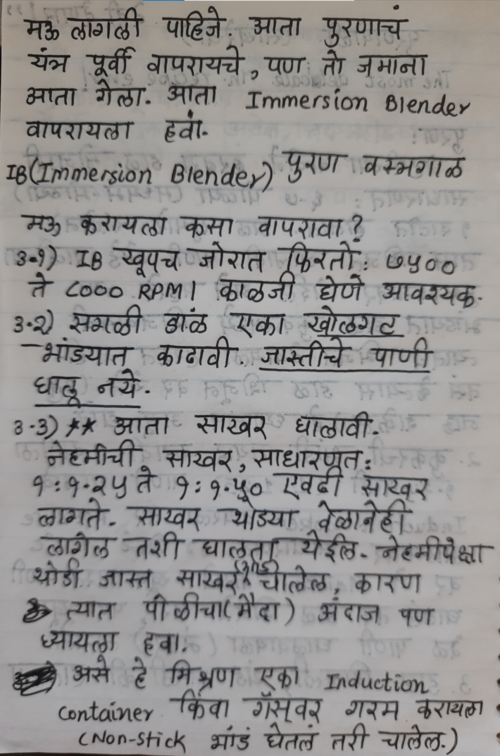
\includegraphics{img/02-s.png}
\end{figure}
\begin{figure}[h!]
    \centering
    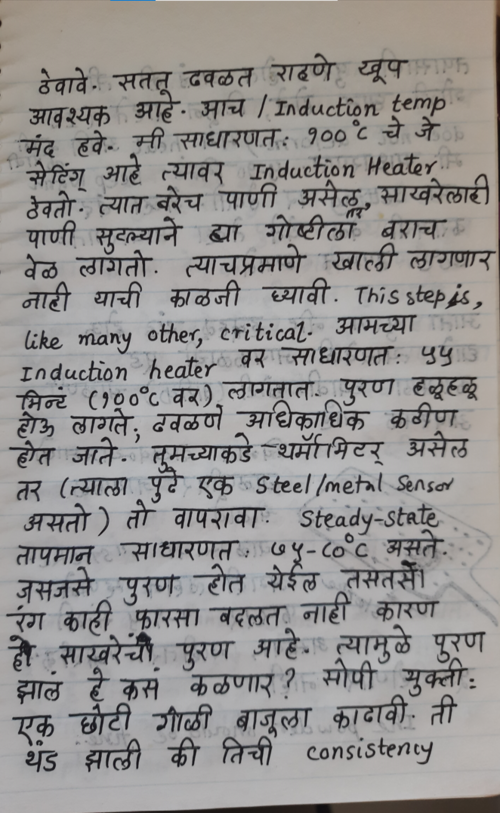
\includegraphics{img/03-s.png}
\end{figure}
\begin{figure}[h!]
    \centering
    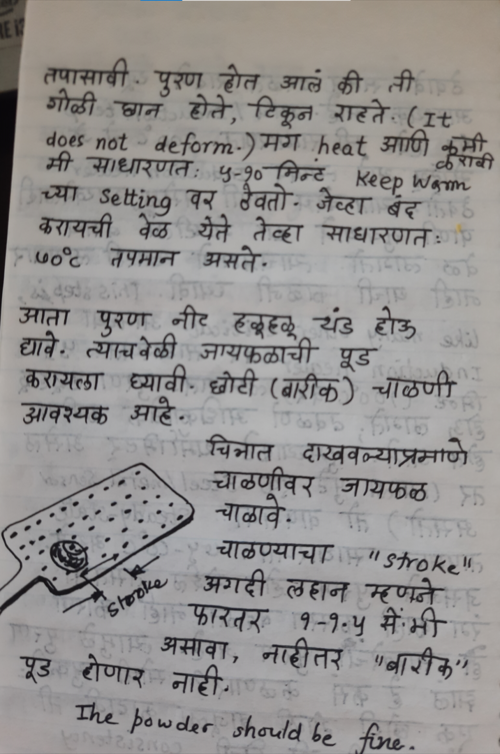
\includegraphics{img/04-s.png}
\end{figure}
\begin{figure}[h!]
    \centering
    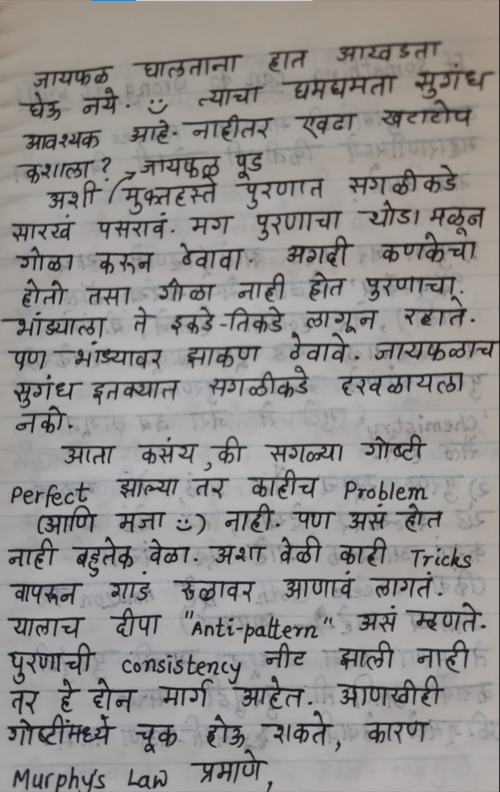
\includegraphics{img/05-s.png}
\end{figure}
\begin{figure}[h!]
    \centering
    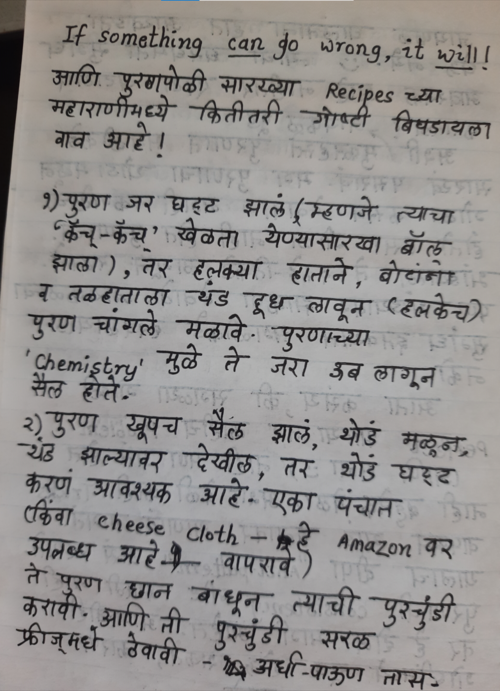
\includegraphics{img/06-s.png}
\end{figure}
\begin{figure}[h!]
    \centering
    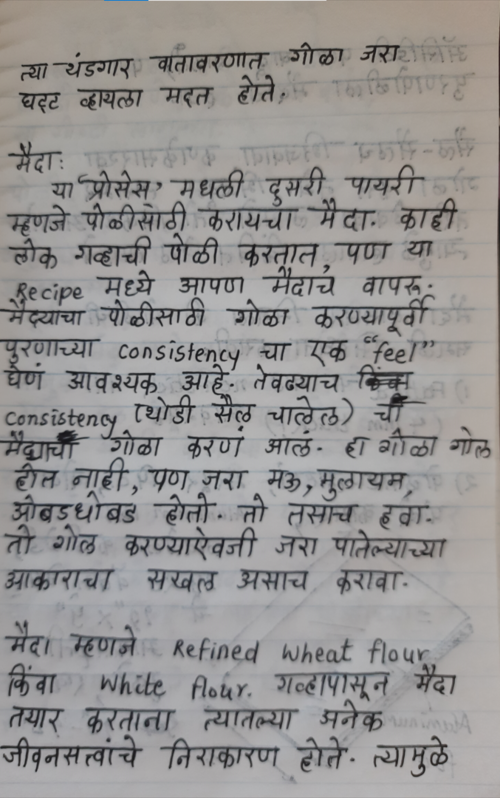
\includegraphics{img/07-s.png}
\end{figure}
\begin{figure}[h!]
    \centering
    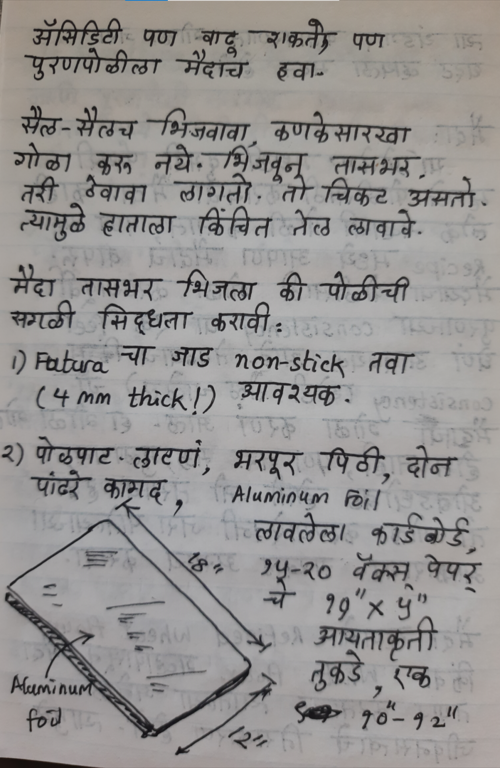
\includegraphics{img/08-s.png}
\end{figure}
\begin{figure}[h!]
    \centering
    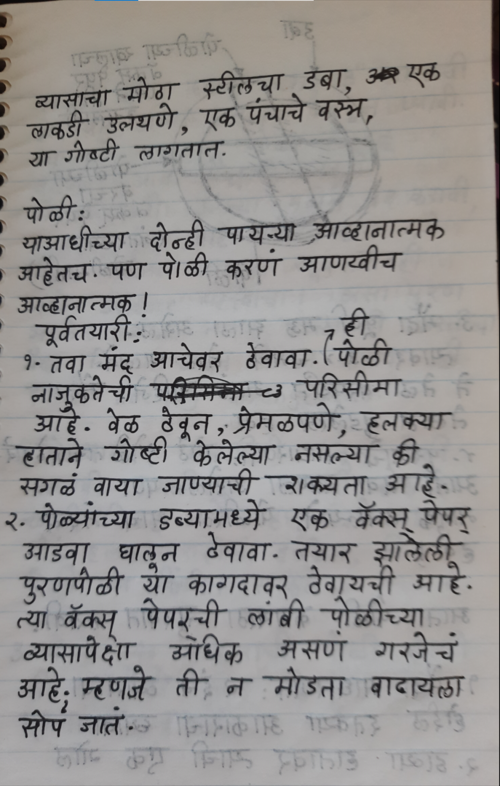
\includegraphics{img/09-s.png}
\end{figure}
\begin{figure}[h!]
    \centering
    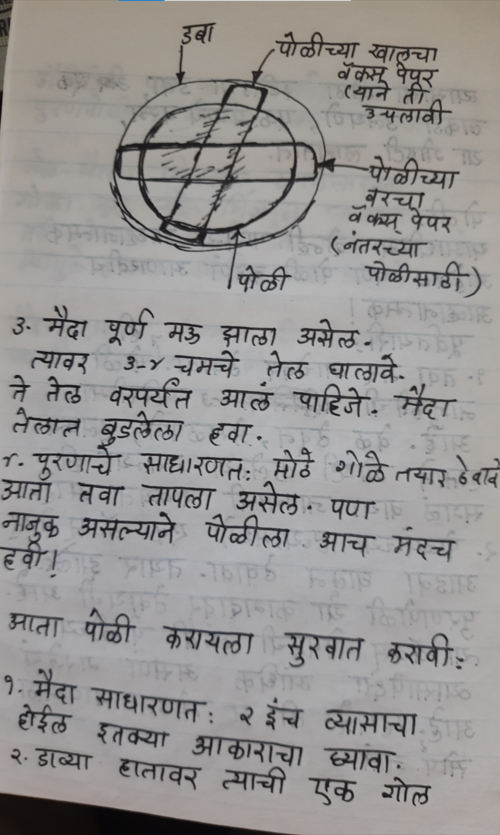
\includegraphics{img/10-s.png}
\end{figure}
\begin{figure}[h!]
    \centering
    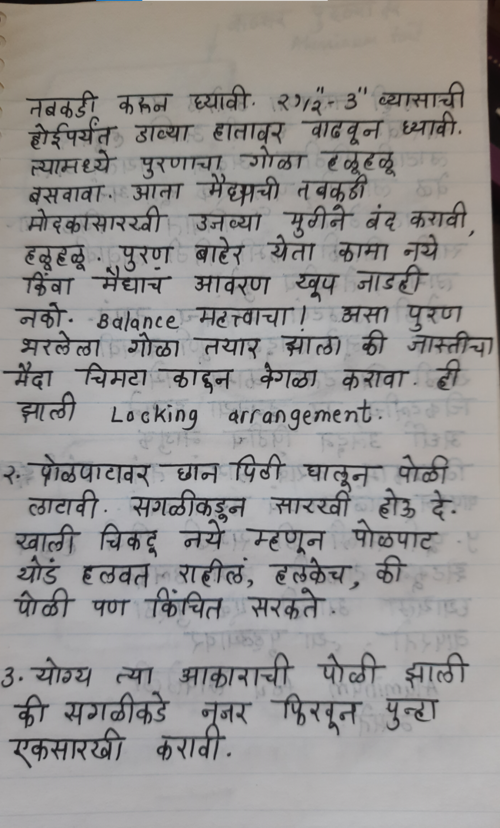
\includegraphics{img/11-s.png}
\end{figure}
\begin{figure}[h!]
    \centering
    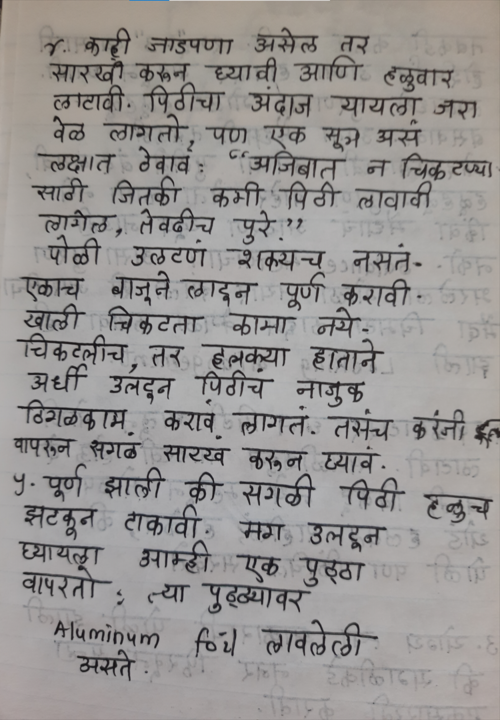
\includegraphics{img/12-s.png}
\end{figure}
\begin{figure}[h!]
    \centering
    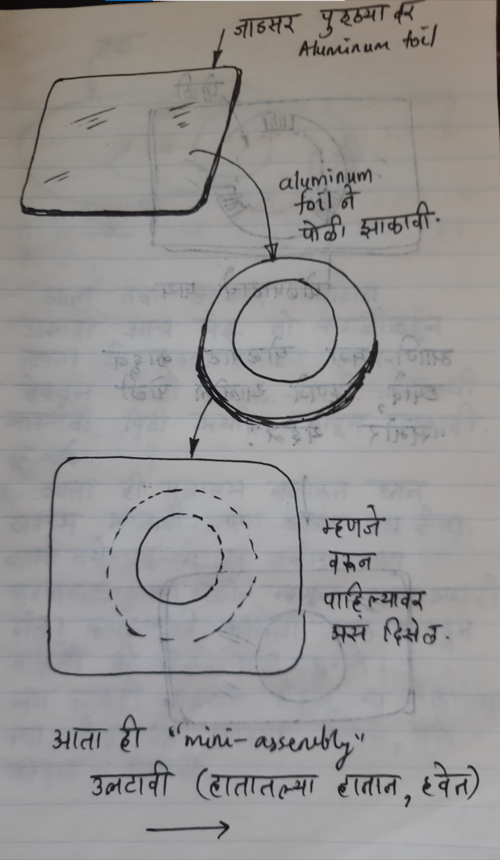
\includegraphics{img/13-s.png}
\end{figure}
\begin{figure}[h!]
    \centering
    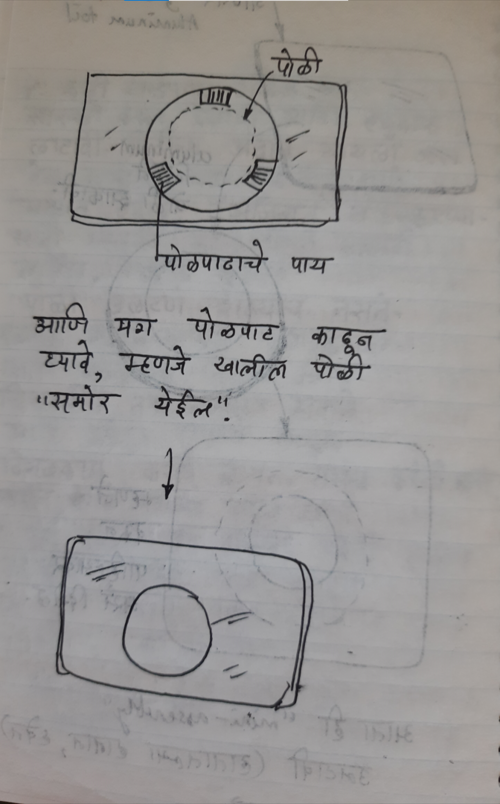
\includegraphics{img/14-s.png}
\end{figure}
\begin{figure}[h!]
    \centering
    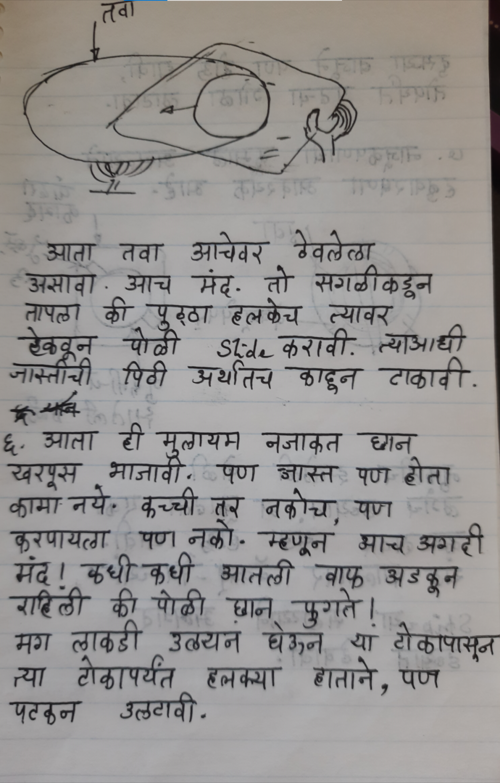
\includegraphics{img/15-s.png}
\end{figure}
\begin{figure}[h!]
    \centering
    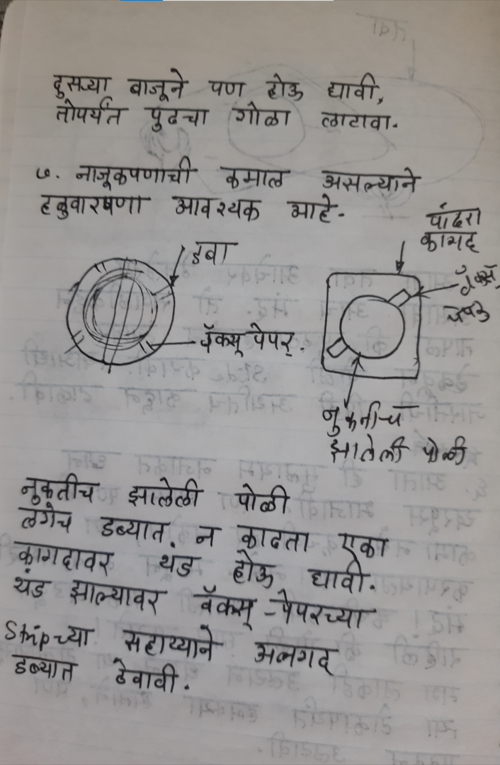
\includegraphics{img/16-s.png}
\end{figure}
\begin{figure}[h!]
    \centering
    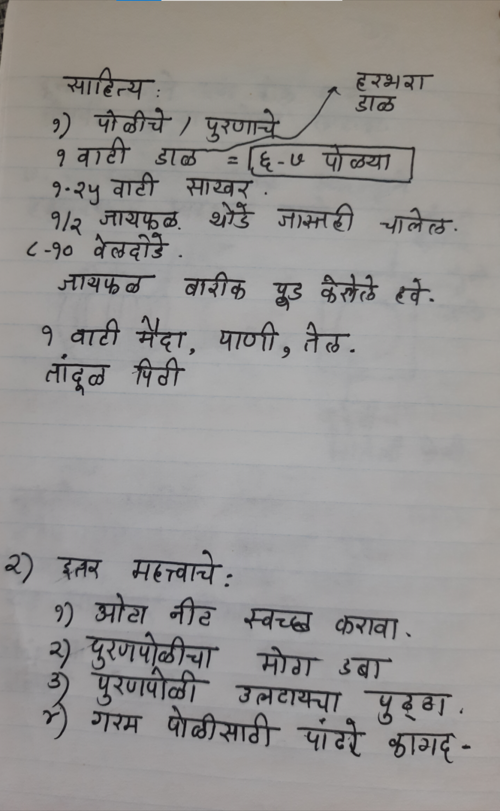
\includegraphics{img/17-s.png}
\end{figure}
\begin{figure}[h!]
    \centering
    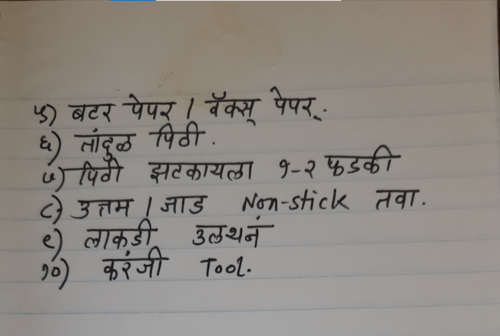
\includegraphics{img/18-s.png}
\end{figure}

\vspace{5mm}
\hrule
\end{document}
